
\chapter{Metric Spaces}\label{ch:metric:spaces}

Prior to this chapter we have developed the theory of vector spaces, dual vector spaces, and the tensor products of these spaces. We defined the relation between these spaces with respect to linear maps. This, in turn, gave further insight on how the basis imposed on a vector space is translated to its dual space. We presented the idea that a tensor could be used to convert one type of object into another. 

In this chapter we see what happens when we \emph{define} an \emph{additional} machine on this structure. This machine is a special tensor called the \textbf{metric}, also known as the \textbf{dot product}, \textbf{inner product}. By defining this structure, we \emph{upgrade} or vector space into what is called a \textbf{metric space}\index{metric space}---a vector space equipped with a metric. This upgrade unlocks our ability to define key ingredients for geometry: length and angle. In turn, this allows us to describe special relativity a language naturally attuned to it.\sidenote{Having come this far, you may see that we have worked hard to build a mathematical machinery. The example of special relativity is our first payoff: it is not that we want to build unnecessarily sophisticated mathematics, it is that building the mathematical machine lets us write actual physical phenomena in a \emph{succinct} language that highlights physical principles. That is: I would rather understand relativity as a unification of space and time under a metric rather than as a cobbled together list of otherwise unrelated rules.}

\section{Metric and Inner Product}

The metric and inner product are so closely related that they are \emph{essentially} the same idea. The \textbf{metric} is a special (0,2)-tensor that we write as
\begin{align}
    g_{ij}\bra{e^i}\bra{e^j} \ .
\end{align}
Often physicists just write the \emph{components} of the metric, $g_{ij}$, and assume that you all agree on the basis.\sidenote{There's more to this. Usually the metric defines for us what a `nice' basis is. When physicists simply write $g_{ij}$ without telling you the basis, it is usually because the \emph{only} nice bases are the components of the metric are the same.} By definition, the components of the metric are symmetric:
\begin{align}
    g_{ij} = g_{ji} \ .
\end{align}

Why should we consider symmetric metrics? Part of the answer is the observation in Section \ref{sec:permutation:symmerty} that symmetric (0,2) tensors remove the ambiguity of having to define which of the metric's lower indices contracts when offered another tensor's upper index. Another post-facto justification is that the way we use the metric to define lengths and angles is naturally symmetric.

\begin{example}
The \textbf{Euclidean metric}\index{Euclidean metric} is
\begin{align}
    g_{ij} = 
    \begin{cases}
        1 &\text{ if } i = j \\
        0 &\text{ otherwise} \ .
    \end{cases}
    \label{eq:metric:euclidean}
\end{align}
When written as an array of numbers, it is simply the identity matrix.\footnote{Though clearly as an object with two lower indices it is a (0,2) tensor, \emph{not} a matrix---which is what we call (1,1) tensors.}
You may wonder if this is the same as the Kronecker $\delta$ from Section~\ref{eq:kronecker:delta}. It may have the same components when written as an array, but it is \emph{not} the same. The Kronecker $\delta$ is a (1,1) tensor, whereas a metric is a (0,2) tensor. They may have the same numerical values of their components, but they are completely different objects.\footnote{Pick your favorite convergent evolution example to use as an analogy. Sharks and dolphins look remarkably similar, even though one is a fish and the other is a mammal.} 

You could write $g_{ij} = \delta^i_j$, but this is a very strange-looking equation since the index heights do not match. That equation is true component wise---meaning ``plug in any values for $i$ and $j$''---but it is not true if you think this is a tensorial relation:
\begin{align}
    g_{ij}\bra{e^i}\bra{e^j} \neq \delta^i_j \ket{e_i}\bra{e_j} \ .
\end{align}
\end{example}

\begin{example}\label{eg:Minkowski:metric}
The metric for Minkowski space (special relativity) is
\begin{align}
    g_{\mu\nu} = \eta_{\mu\nu}
    =
    \begin{cases}
    \pp 1 & \text{if } \mu=\nu = 0\\
    -1 & \text{if } \mu=\nu > 0\\
    \pp 0 & \text{otherwise}
    \end{cases} \ .
    \label{eq:Minkowski:metric}
\end{align}
We introduce some conventional notation. First, the special relativity metric is called $\eta_{\mu\nu}$ whereas the general relativity (with gravity) metric is called $g_{\mu\nu}$. Second, we distinguish between time and space by indexing time as $\mu=0$. In order to remind us that the indices start with zero, we use lowercase letters from the middle of the Greek alphabet ($\mu, \nu$) instead of $i,j$.

About a quarter of physicists use this form of the metric. This tribe includes nearly all particle physicists. Another quarter or so use the convention where $\eta_{\mu\nu}^\text{grav.} = -\eta_{\mu\nu}$. This group includes gravitational physicists and formal theorists (what we used to call string theorists). The other half could not care less about the metric of spacetime. 
\end{example}

From the metric one can define the \textbf{inner product}\index{inner product}, which in Euclidean space is what we call a \textbf{dot product}\index{inner product}. This is a function that uses the metric to take in two vectors to return a number:\sidenote{You would be correct in wondering how this is at all different from the metric itself. From the linear map perspective, any (0,2) tensor is \emph{defined} to be a function that takes two vectors and returns a number, $V\times V \to \#$. In this sense, the inner product is \emph{literally} the same as the metric. However, conventionally colleagues say \emph{metric} to mean the components and \emph{inner product} to mean the function. By now we all agree that these really encode same thing.}
\begin{align}
    \la \vec{v},\vec{w} \ra = g(\vec{v},\vec{w})
    = g_{ij} v^i w^j \ .
\end{align}
Because of the symmetry of $g_{ij}$, we have
\sidenote{By the way, please appreciate that we now freely moving between our different conventions for referring to tensors---$v^i$, $\vec{v}$, $\ket{v}$---based on whichever is \emph{most convenient} for the case at hand. This avoids cumbersome notation, like writing an inner product using ket notation, for example: $\la \ket{v}, \ket{w} \ra$. }
\begin{align}
    \la \vec{v}, \vec{w} \ra = \la \vec{w}, \vec{v} \ra \ .
\end{align}



\begin{exercise}
Show that the components the metric are easily (perhaps \emph{tautologically}\footnote{This is a mathematicians way of saying `obvious.' In fact, it is more than that. It is something that Anthony Zee calls ``more obvious than obvious'' (I think I picked this up from his quantum field theory book). What this means is that the fact is so `by definition' self-apparent that any attempt to explain it will only obfuscate the matter.}) expressed as inner products of the basis vectors:
\begin{align}
    g_{ij} = \la \bas{e_i}, \bas{e_j}\ra \ .
\end{align}
\end{exercise}

There is one more practical requirement for a metric: the metric is invertible. Another way of saying this is that it is \emph{non-degenerate}. 

\section{A tool to define length}
\label{sec:machine:to:make:row:vectors}

The \textbf{length}\index{length} of a vector $\vec{v}$ is defined by
\begin{align}
 |\vec{v}|^2  
 = \la \vec{v},\vec{v} \ra 
 = g_{ij}v^iv^j
 \ .
 \label{eq:lenght:in:terms:of:metric}
\end{align}

\begin{exercise}
Observe that if the metric had any antisymmetric part, then it would cancel in its contribution to the length. 
\end{exercise}

\begin{example}
For the case of the Euclidean metric \eqref{eq:metric:euclidean}, the length is exactly what one expects from plane geometry: a vector is some arrow starting at the origin whose length is determined by an application of the Pythagorean theorem. One obvious observation is that any Euclidean vector with non-zero components has non-zero length.
\end{example}

\begin{example}
For the case of the Minkowski metric \eqref{eq:Minkowski:metric} in (1+1)-dimensions\footnote{It is conventional to write the dimension of Minkowski space as a sum of the time and space dimensions.} the length of a vector is:
\begin{align}
    |\vec{v}|^2 = (v^0)^2 - (v^1)^2 \ .
    \label{eq:minkowski:length:2d}
\end{align}
Unlike Euclidean space, you can have a Minkowski space vector, say 
\begin{align}
    v^\mu = 
    \begin{pmatrix}
        7\\
        7
    \end{pmatrix} \ ,
\end{align}
that has obviously non-zero components but has \emph{zero length}. We call these \textbf{null vectors}\index{null vector}. In fact, any such vector in (1+1)-dimensional Minkowski space with $|v^0| = |v^1|$ is a null vector.
\end{example}

\begin{exercise}
Argue that in any metric space, the length of the vector is a square root of some expression that is quadratic in the components of the vector. In other words, there can be no metric spaces where something weird happens like
\begin{align}
    |\vec{v}| = \sqrt[3]{(v^1)^2 + v^1v^2 - (v^2)^2}
\end{align}
or perhaps
\begin{align}
    |\vec{v}| = (v^1)^3 - (v^2)^2 \ .
\end{align}
You can argue this purely based on the mathematical definition of a metric space. As a physicist, these definitions also make no sense the moment you think about units.
\end{exercise}

Because the length is just a number, we can rescale any vector by its length to get a \textbf{unit vector}\index{unit vector}, a vector with unit length:
\begin{align}
    \hat{\vec{v}} \defeq \frac{\vec{v}}{|\vec{v}|} \ .
\end{align}
We say that vectors with unit length are \textbf{normalized}\index{normalized}. 


\section{A tool to define angles}

Given two vectors $\vec{v}$ and $\vec{w}$, the \textbf{angle}\index{angle} between these vectors is defined by
\begin{align}
    \cos\theta = \frac{\la \vec{v}, \vec{w} \ra}{|\vec{v}| |\vec{w}|}
    =
    \la \hat{\vec{v}}, \hat{\vec{w}} \ra \ .
    \label{eq:cos:theta:angle:defined:metric}
\end{align}
Because the metric and inner product are symmetric, the cosine of the angle between two vectors does not depend on the order of the vectors.\sidenote{There is a notion of the angle from $\vec{v}$ to $\vec{w}$ being negative that of the angle from $\vec{w}$ to $\vec{v}$. This is called orientation. However, because cosine is an even function, $\cos\theta = \cos(-\theta)$, and so the definition for the cosine of the angle in terms of the inner product is robust. One just has to remember that inverting the cosine has multiple solutions.}

\begin{exercise}
Show that the angle between two vectors is independent of the length of the vector. 
\end{exercise}

\begin{exercise}
Show that in (1+1)-dimensional Minkowski space two vectors may each be \emph{null} (zero length), $\la \vec{v},\vec{v}\ra =0$, but may have non-zero angle with one another. Give an explicit example.  \textsc{Hint}: the condition for a vector to be null has two solutions. Check the inner product of the two.
\end{exercise}


\section{A tool to lower indices}
\label{{sec:machine:to:make:row:vectors}}

The following observation is, by far, the most common way to think about the metric:
\begin{quote}
The metric is a machine that takes an upper index and returns a lower index.
\end{quote}
That this is true is obvious: any (0,2) tensor is a linear map from vectors to dual vectors. We know this from the discussion in Example~\ref{eg:maps:between:product:spaces}. Here's how it works in full tensorial glory:
\begin{align}
    g_{ij}\bra{e^i}\bra{e^j} \; v^k \ket{e_k}
    &= 
    g_{ij}v^k \delta^j_k \; \bra{e^i}
    =
    g_{ij}v^j\; \bra{e^i}
    % \defeq v_i \bra{e^i} 
    \ .
    \label{eq:metric:lowering:full:tensor}
\end{align}
\begin{exercise}
Use the fact that the metric is symmetric to show that one obtains the same result if we contract the $\bra{e^i}$ with the $\ket{e_k}$ rather than the $\bra{e^j}$ with the $\ket{e_k}$ in \eqref{eq:metric:lowering:full:tensor}. That is:
\begin{align}
    g_{ij}\bra{e^i}\bra{e^j} \; v^k \ket{e_k}
    = 
    g_{ij}\bra{e^j} \; v^k \la {e^i}\mid {e_k}\ra \
    =
    g_{ji}v^i \bra{e^j}
    \ .
\end{align}
\end{exercise}

What is significant here is that when we define the metric space, we require that everyone agrees on the definition of the metric. That means that given a vector $\ket{v} = v^i\ket{e_i}$ in a metric space with a metric $g_{ij}\bra{e^i}\bra{e^j}$,\sidenote{Usually we would just say ``given a vector $v^i$ and a metric $g_{ij}$'' and leave the tensor basis implicit.} we can make the following \emph{definition}:
\begin{align}
    v_i \defeq g_{ij}v^j \ .
\end{align}
Let us spell out exactly what is going on:
\begin{enumerate}
    \item Until this point, there was \emph{no object} whose component carries a single lower index. We only assumed that you have a vector (one upper index) and a metric (two lower indices). 
    \item Now we have defined a new object $v_j$ who shares the same variable name as the vector $v^i$, except with a lower index.
    \item This lower-object version of $v^i$ is defined to be the contraction of $v^i$ with the metric. It is completely expected that this contraction gives an object with a lower index, but usually we would call it $(gv)_i = g_{ij}v^j$.
    \item Since there is no other object that (a) has the variable name $v$ \emph{and} (b) carries a single lower index, we choose to \emph{define} $v_i = g_{ij}v^j$. 
    \item Because we are in a metric space, we assume everyone knows what the metric is. That means there is no ambiguity about how to form $v_i$ from $v^j$: it is \emph{understood} that we use the metric. So as a shorthand, we stop writing the metric explicitly.
\end{enumerate}

We generalize this to lower any index on a tensor with an upper index:
\begin{newrule}[Lowering indices with the metric]
Suppose you have a tensor whose components include some upper index, say $T\aij{ijk}{\ell}$. If you see a tensor with the \emph{same variable name} but with that index lowered, then it is \emph{understood} that this means
\begin{align}
    T\aij{ij}{k\ell} \defeq g_{km}T\aij{ijm}{\ell} \ .
\end{align}
\end{newrule}
Now that we have a rule to lower indices, please be careful that you must \emph{preserve the order of the indices}! 
\begin{example}
If you have a tensor with components $T\aij{ijk}{\ell}$, then $T\aij{ij}{k\ell}$ is different from $T^{i\phantom{j}k}_{\phantom{i}j\phantom{k}\ell}$. Explicitly:
\begin{align}
    T\aij{ij}{k\ell} = g_{km}T\aij{ijm}{\ell}
    \neq
    T^{i\phantom{j}k}_{\phantom{i}j\phantom{k}\ell}
    = g_{nj}T\aij{ink}{\ell} \ .
\end{align}
\end{example}
\begin{example}
We can lower multiple indices. Suppose you have a tensor whose components include some upper index, say $T\aij{ijk}{\ell}$. Then we have an implicit definition for the tensor with all of its indices lower:
\begin{align}
    T_{ijk\ell} = g_{im}g_{jn}g_{kp}T\aij{mnp}{\ell} \ .
\end{align}
\end{example}

\section{Is this a transpose?}

At this point, it is natural to draw on your familiarity with matrix algebra and to think that the metric seems to ``tip over'' a column vector and turn it into a row vector. You may ask, as the popular meme in Figure~\ref{fig:is:this:a:transpose}, whether we are defining a transpose. We are \emph{not}.
\begin{marginfigure}%[th]
    
\includegraphics[width=\textwidth]{figures/IsThisTranspose.jpg}
    \captionsetup{font={scriptsize,sf}}
    \caption{The metric is \emph{not} a transpose. ``Is This a Pigeon'' meme via \url{https://imgflip.com/i/8nc9fd}.}
    \label{fig:is:this:a:transpose}
\end{marginfigure}

\begin{example}[Tipping over a column vector?]
In \emph{Euclidean space}, lowering an index with the metric is apparently equivalent to ``tipping over'' the column vector. As an explicit example, consider a vector
\begin{align}
    \vec{v}=
    \begin{pmatrix}
        v^1\\v^2\\v^3
    \end{pmatrix}
    =
    \begin{pmatrix}
        1\\2\\3
    \end{pmatrix} \ .
\end{align}
By acting on this vector with the metric, we produce a row vector with components $v_i = g_{ij}v^j$. Using the trivial Euclidean metric \eqref{eq:metric:euclidean}, this says that the component with the upper index is the same as the component with the lower index:
\begin{align}
    \row{v} = 
    \begin{pmatrix}
        v_1 & v_2 & v_3
    \end{pmatrix}
    =
    \begin{pmatrix}
        1 & 2 & 3
    \end{pmatrix} \ .
\end{align}
So indeed, it looks like we just knocked the column vector over and it is now lying down flat---but the components are all the same. 

In any other space, the numerical values of the row vector are rather different. Consider the Minkowski metric \eqref{eq:Minkowski:metric}. Once again, we start with a column vector with the same components---though in line with the Minkowski convention in Example~\ref{eg:Minkowski:metric} we index starting from 0:
\begin{align}
    \vec{v}=
    \begin{pmatrix}
        v^0\\v^1\\v^1
    \end{pmatrix}
    =
    \begin{pmatrix}
        1\\2\\3
    \end{pmatrix} 
    \ .
\end{align}
As before, the components of the row vector are $v_\mu = g_{\mu\nu}v^\nu$, where the content of this equation is \emph{identical} to $v_i = g_{ij}v^j$ except that we use the physics convention of writing spacetime indices with Greek indices. Then our row vector has \emph{different} components:
\begin{align}
    \row{v} = 
    \begin{pmatrix}
        v_0 & v_1 & v_1
    \end{pmatrix}
    =
    \begin{pmatrix}
        1 & -2 & -3
    \end{pmatrix} \ .
\end{align}
\end{example}

\begin{exercise}
Consider a 2-dimensional metric space whose metric contains---rather annoyingly---off-diagonal elements:
\begin{align}
    g_{ij} = \begin{pmatrix}
        g_{11} & g_{12} \\
        g_{21} & g_{22}
    \end{pmatrix}
    =
    \begin{pmatrix}
        1 & \varepsilon \\
        \varepsilon & 1
    \end{pmatrix} \ ,
\end{align}
for some constant $\varepsilon$. If you have a vector $\vec{v} = v^i \bas{e}_i$, what are the components of the corresponding dual vector $\row{v} = v_i \rbas{e}^i$? Make sure that this matches the Euclidean case when $\varepsilon\to 0$.
\end{exercise}

So let us emphasize: using the metric to lower an index is \emph{not} a transpose. There is a proper definition of transpose for matrices, but there is no such thing as the `transpose of a vector.' One feature that is useful from that otherwise incorrect notion is that the tensor with a metric-lowered index physically encodes the same content as the original tensor. In this way, it is the `same' tensor.

\begin{bigidea}[Is it a `different' tensor?]
Conceptually, \emph{in a metric space}, you should think of $\ket{v} = v^k \ket{e_k}$ and $\bra{k} = v_k \bra{e^k}$ as the `same' essential object, but with different components reflecting whether the object is being used as a vector or a dual vector. This is usually the case in physical applications. For example, in relativity the four-momentum---a vector containing the energy and the three spatial momenta---is a vector. The dual vector may have different components---the metric introduces minus signs on the spatial components---but we understand it to encode the same ``energy and the three spatial momenta'' as the upper-indexed object.
\end{bigidea}



\begin{example}
The fact that the Euclidean metric is so boring is part of the reason why we often take it for granted. Many first-time learners of linear algebra (done properly) are confused why row vectors and column vectors are treated differently. In these lectures we emphasized that when you only have a vector space and not a metric space, you cannot convert between vectors and row vectors. The vector spaces that we grow up with---Euclidean three-space---implicitly have a metric. After all, you grew up `knowing' how to take the length of a vector or the angle between vectors.\footnote{Of course, many of us also grow up with the completely wrong idea that positions are vectors.} 

The challenge here is to realize that when we were young, we had been \emph{assuming} the existence of a metric without explaining that it is an additional structure that we can choose---as in the case of Minkowski space. I grew up in a household where every meal came with rice. It never occurred to me that there might be other starches that could form the base of a meal. The first time I went to a grade school friend's house for dinner and we had mashed potatoes---but no rice---completely blew my mind. 
\end{example}

In this course the primary example of a non-Euclidean metric is Minkowski space and special relativity. General relativity---which is special relativity plus gravity---have different kinds of spacetime metric.\sidenote{In fact, the metric itself is a dynamical variable that responds to energy.} In quantum mechanics our vector space of quantum states has what is essentially a Euclidean metric, though the space is formally complex.\sidenote{Every time we say `number' we allow for the number to contain some imaginary part.} The other place where unusual metrics show up in physics are more abstract vector spaces. My favorite example of this what are the vector spaces of generalized rotations.\sidenote{Unfortunately this topic is rather outside the scope of our course.}


\section{Example: Polar Coordinates}
\label{sec:polar:coordinates}

In the bundle picture of Chapter~\ref{ch:bundles}, we said that each tangent plane is a different vector space. Polar coordinates on Euclidean space is an example where this bundle structure shows up in a space that is \emph{not} actually curved, but is described readily with curved for the base space. 

\textbf{Curvilinear coordinates}\index{curvilinear coordinates} are coordinates grids that are not straight lines, the way that the Cartesian $x$--$y$ plane is a grid. Polar coordinates replace $(x,y)$ with $(r,\theta)$. Here $r$ is the distance from the origin and $\theta$ is the angle from the positive $x$-axis. These are coordinates on the \emph{base space}, which is not a vector space.
 
This example is surprisingly subtle. The take-away is that the metric in polar coordinates is
\begin{align}
    g_{ij} = 
    \begin{pmatrix}
        g_{rr} & g_{r\theta} \\
        g_{\theta r} & g_{\theta\theta}    
    \end{pmatrix}
    =
    \begin{pmatrix}
        1 & \\
        & r^2
    \end{pmatrix} \ .
    \label{eq:polar:metric}
\end{align}
The bottom right component is not one, but rather the radial coordinate on the base space. 

The surprising piece in \eqref{eq:polar:metric} is that $g_{\theta\theta} = r^2$. This means that the metric changes as you move further away from the origin of the coordinate space. This is in contrast to the Euclidean metric whose components are proportional to the identity no matter where you happen to be.

This should not surprise us. We know that the same \emph{angular displacement} $\Delta \theta$ corresponds to a different traversed circumference depending on the radius. If you are close to the origin, then a displacement of $\Delta\theta$ is not particularly far. If you are far from the origin, then a displacement of $\Delta\Theta$ can be huge, see Fig.~\ref{fig:polar:displacement}.\footnote{This sometimes shows up in the ``paradox'' (it is not a paradox) that ``shadows travel faster than the speed of light.''} From a physics perspective, you could have guessed this from pure dimensional analysis: $\Delta \theta$ is dimensionless. If you want your metric to output a squared distance, then you need something with dimensions of length---the only plausible candidate is $r^2$. This is illustrated nicely in the \emph{Calvin and Hobbes} comic in Fig.~\ref{fig:CH:record:player}.




\begin{figure}[tb]
    \centering
    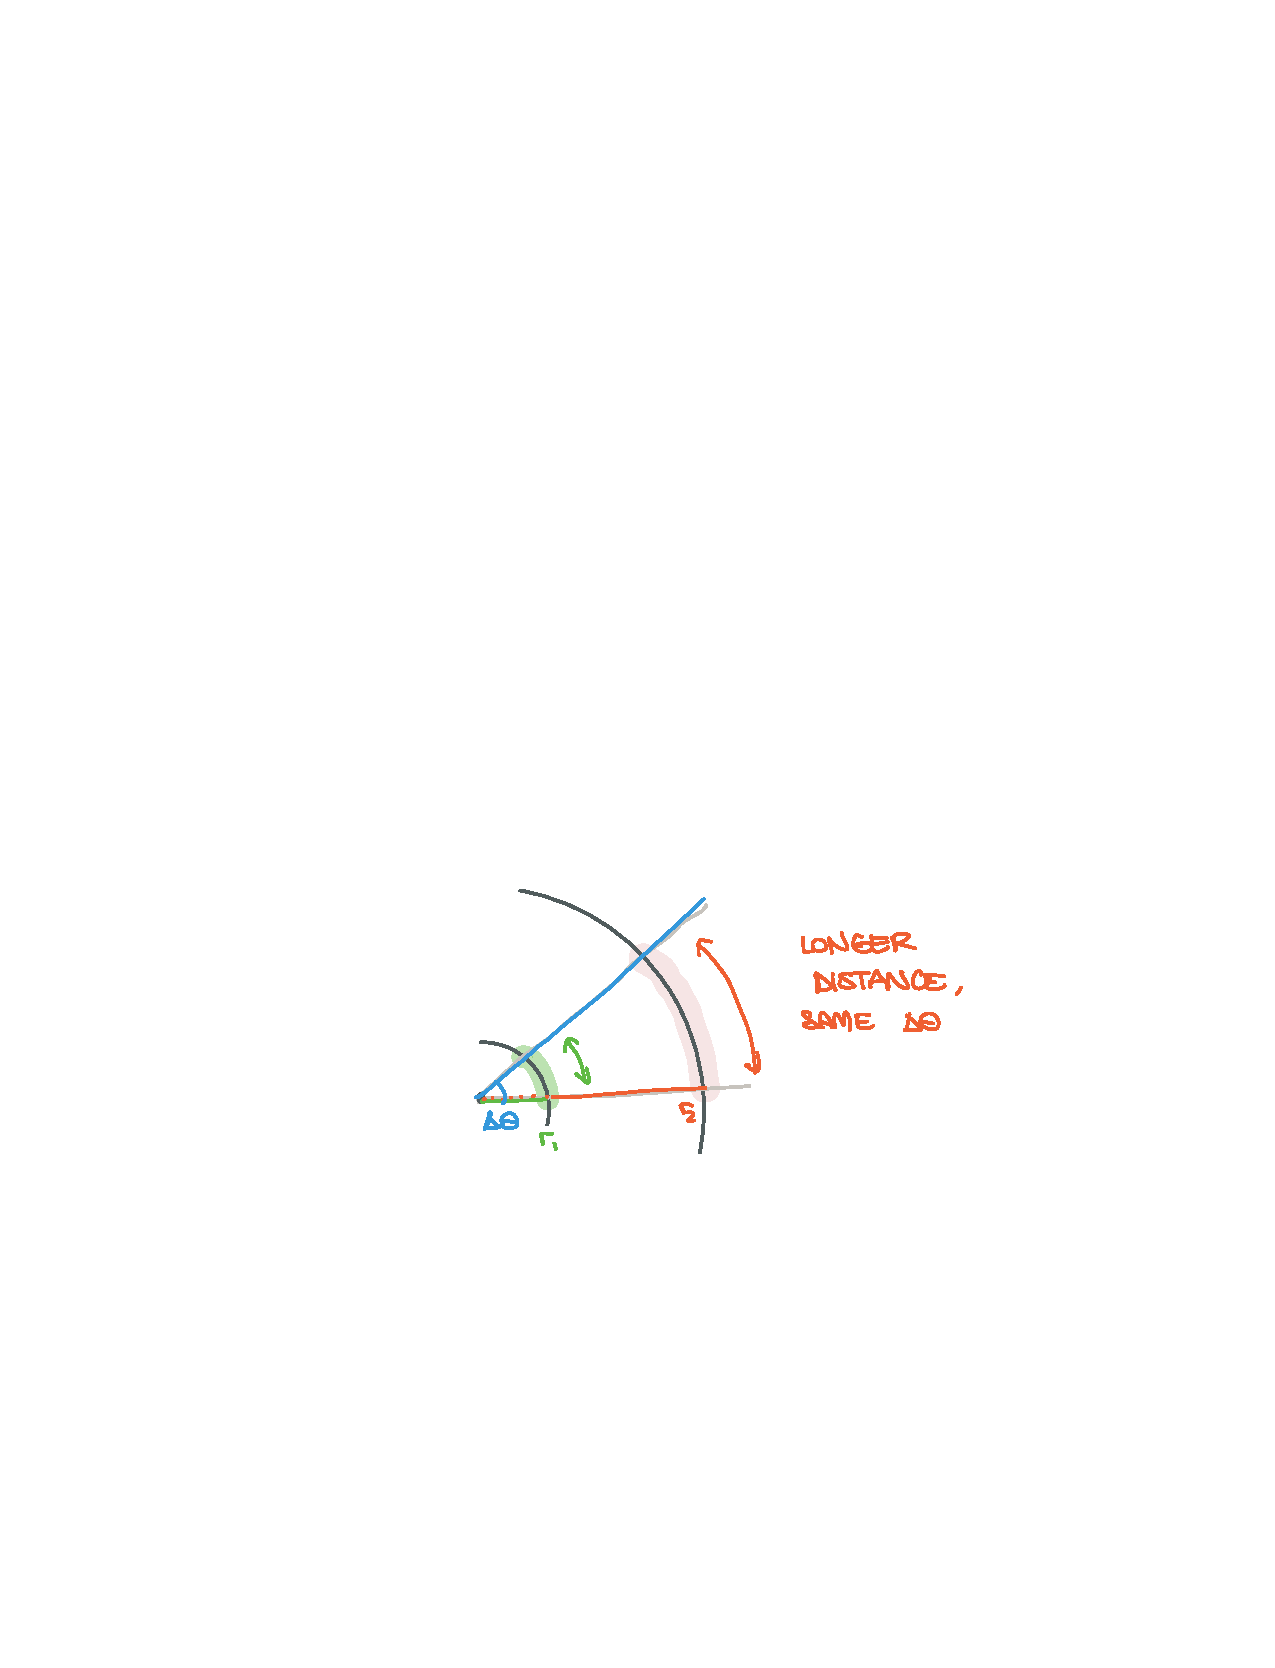
\includegraphics[width=.4\textwidth]{figures/polar_longer_distance_dtheta.pdf}
    \caption{The meaning of the $g_{\theta\theta} = r^2$ is related to the idea that the distance traversed along a circle for a displacement $\Delta\theta$ depends on the radius of the circle.}
    \label{fig:polar:displacement}
\end{figure}

\begin{figure}[tb]
    \centering
    
\includegraphics[width=\textwidth]{figures/calvin_and_hobbes_record.jpg}
    \caption{\emph{Calvin and Hobbes}, ``Record Player,'' by Bill Watterson, 5 June 1990. Image from \url{https://www.gocomics.com/calvinandhobbes/1990/06/05}. If you have never heard of a record player than look it up.}
    \label{fig:CH:record:player}
\end{figure}
% Also: mechanical integrator: https://www.youtube.com/watch?v=s-y_lnzWQjk
% Also: differential steering: https://www.youtube.com/watch?v=yYAw79386WI

\begin{example}
While this is not really relevant for linear algebra, there are a few neat ways in which the difference between angular and linear velocity show up. One is the mechanical integrator\footnote{\url{https://www.youtube.com/watch?v=s-y_lnzWQjk}}, and another is differential steering\footnote{\url{https://www.youtube.com/watch?v=yYAw79386WI}}. 
\end{example}


\begin{exercise}\label{ex:polar:location:dependence}
Consider the vector $\vec{v} = 3\bas{e}_r - (\pi/4)\bas{e}_\theta$ located at the point $(r,\theta)=(2, \pi/6)$. Find the length of this vector, $|\vec{v}|$ using the polar coordinate metric \eqref{eq:polar:metric}. Observe that for this problem we have to specify the location of the vector---a location on the base (coordinate) space. 
\end{exercise}



\begin{figure}[tb]
    \centering
    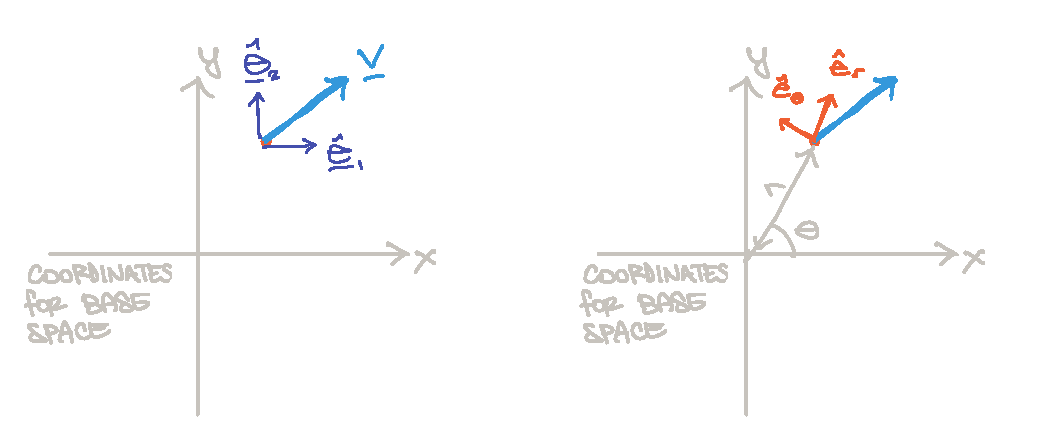
\includegraphics[width=.8\textwidth]{figures/PolarBasis.pdf}
    \caption{Consider a point in $\RR^2$ and some vector $\vec{v}$ that represents the velocity of a particle at that point. We can write $\vec{v}$ in the usual Cartesian basis (left), or in the polar basis (right). Both bases are orthonormal, but they are oriented differently.}
    \label{fig:polar:coordinate:vs:vector:space}
\end{figure}


\begin{figure}[tb]
    \centering
    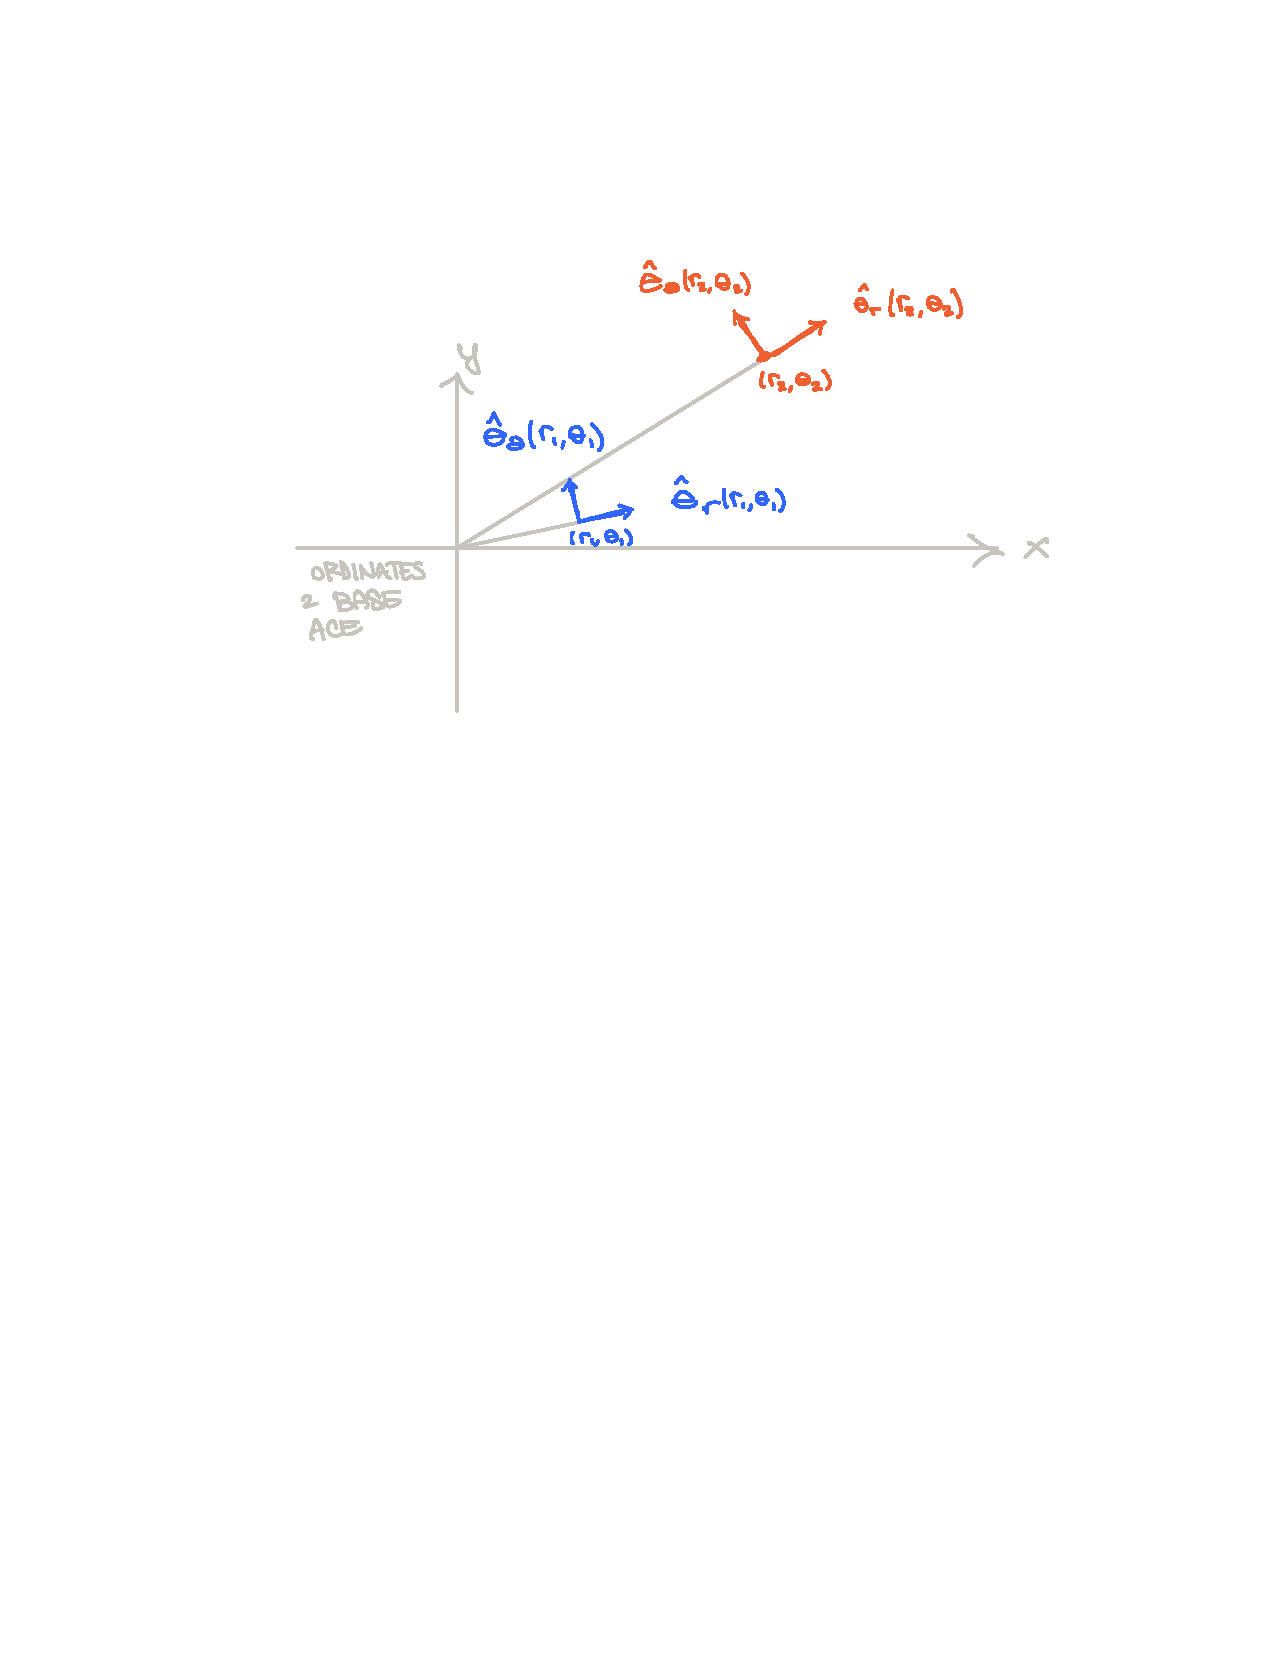
\includegraphics[width=.6\textwidth]{figures/polar_different_orientation.pdf}
    \caption{The basis vectors are a basis for potential velocities of a particle at that point. The orientation of the polar coordinate basis vectors depends on the point at which we are using them. }
    \label{fig:polar:coordinate:vs:vector:space:two:points}
\end{figure}


When a metric that differs from the identity\footnote{By which we mean a metric whose components are different from the components of the identity matrix.} we should suspect that we may be in a \emph{curved space}. For example, the surface of the Earth is a curved space whose metric in spherical coordinates is
\begin{align}
    g_{ij} = 
    \begin{pmatrix}
        g_{\theta\theta} & g_{\theta\phi}\\
        g_{\phi\theta} & g_{\phi\phi}
    \end{pmatrix}
    =
    \begin{pmatrix}
        r^2 & \\
        & r^2 \sin^2\theta
    \end{pmatrix} \ ,
    \label{eq:metric:surface:of:sphere}
\end{align}
where $r$ is the radius of the Earth. However, it is not true that all `funny looking metrics' imply that the underlying space is curved. In the polar coordinate example of this subsection, the space itself is the same two-dimensional Euclidean space that we are used to. All we have done is changed coordinates. We see that a funny looking metric may mean that the space is curved, or it may mean that our coordinate system is curved (that is, \emph{curvilinear}). 


\begin{exercise}
Prove \eqref{eq:metric:surface:of:sphere}. You may need to review your trigonometry and draw the sphere carefully. Observe that this is a two-dimensional metric space for the surface of the sphere. There is no radial vector. Feel free to derive the three-dimensional spherical coordinate metric that includes the radial direction. 
\end{exercise}

\subsubsection{The polar basis}

Let us check the orthonormality of the polar basis at some point, $(r,\theta) = (3,\pi/4)$. The fact that $\bas{e}_r$ and $\bas{e}_\theta$ are orthogonal should be obvious: one points in the radial direction and one points in the polar direction---these are orthogonal directions by definition. Another way of seeing this is that the metric is diagonal. 
\begin{exercise}
Confirm that if a metric is diagonal, then the basis vectors are obviously orthogonal. 
\end{exercise}
The length of the $\bas{e}_r$ vector is also normalized since $\langle \bas{e}_r, \bas{e}_r\rangle = g_{rr} = 1$. What about the length of $\vec{e}_\theta$? This is a vector corresponding to a shift of one unit in the $\theta$ direction. We have
\begin{align}
    \langle \vec{e}_\theta, \vec{e}_\theta \rangle = g_{\theta\theta} = r^2 \ .
\end{align}
Well that's unusual. If we are at $r=3$, then $\langle \vec{e}_\theta, \vec{e}_\theta \rangle = 9$. This means that the normalized basis vector is
\begin{align}
    \bas{e}_\theta = \frac{\vec{e}_\theta}{r} \ .
\end{align}
This makes sense because a `shift of one unit in the $\theta$ direction' is a much larger step the further away you are from the coordinate origin, as we saw in Fig.~\ref{fig:polar:displacement}.










\section{Inner Product, pre-loaded}\label{eq:inner:product:pre:loaded}

The inner product\sidenote{Which, again, is really the same thing as the metric but often is written out with angle brackets.} is a linear function from $V\times V \to \#$. This is a good place to review the linear map picture of tensors from Section~\ref{sec:linear:maps}. We recognized in that section that a linear map from $V\times V \to \#$ could equivalently be understood as a linear map from $V \to V^*$. In fact, this is precisely what it means to `lower an index' and convert a vector into a dual vector.

From the perspective of linear functions,\sidenote{Here we shift again to a different notation to make the idea clear---but everything we write could equivalently be written in bra-ket notation.} the dual vector that we produce from a vector $\vec{v}$ is 
\begin{quote}
the inner product with one of the slots pre-filled with $\vec{v}$.
\end{quote}
To let this sink in, let us write it out mathematically:
\begin{align}
    % \row{v} \defeq \la \vec{v}, \Vtextvisiblespace[1em]{}\, \ra \ .
    \row{v} \defeq \la \vec{v}, \slot{}\, \ra \ .
    \label{eq:dual:vec:is:pre:filled:inner:product}
\end{align}
Here we have written a space, \Vtextvisiblespace[1em]{} to mean \emph{ put in the argument of the linear function $\row{v}$ in here}. In other words, the \emph{dual vector} $\row{v}$ acts on some other vector $\vec{w}$ as
\begin{align}
    \row{v}\left(\ket{w}\right)
    =
    \la \vec{v}, \vec{w} \ra \ .
    \label{eq:row:vector:inner:product}
\end{align}
This means that $\row{v}$, the row-vector version of $\vec{v}$, is a linear function from $V\to \#$ in the sense that you can feed it any vector $\vec{w}$ and it returns $\la \vec{v}, \vec{w}\ra$, which is a number. Linearity is guaranteed because the inner product $\la \Vtextvisiblespace[1em]{}\,,\, \Vtextvisiblespace[1em]{} \ra $ is linear in each argument.\sidenote{In case you forgot, this means that $\row{v}(\alpha \vec{a} + \beta \vec{b}) = \alpha \row{v}\vec{a} + \beta\row{v}\vec{b}$.}
\begin{exercise}
Rewrite everything in this section using bra-ket notation. 
\end{exercise}


\section{Poetic Notation}

In bra-ket notation, there are two very similar expressions: the inner product $\la \vec{w}, \vec{v} \ra$ and the action of a bra and a ket as linear operators: $\row{w}\vec{v} = \la w \mid v\ra$. \emph{Formally} these are different things:
\begin{itemize}
    \item $\la \vec{w}, \vec{v} \ra$ is an inner product. This means that you have two vectors and you want to combine them to get a number. This requires that you have a metric.
    \item $\la w \mid v\ra$ is the definition of the dual relationship between row vectors and dual vectors: they are linear functions of one another. This means that you take one vector $\vec{v} = \ket{v}$ and one row vector $\row{w} = \bra{w}$ and you combine them in the only way that you can to form a number. This does \emph{not} require a metric and was something that we already defined in a regular old vector space.
\end{itemize}

\emph{Practically}, on the other hand, these are deeply connected and the $\la \Vtextvisiblespace[1em]{}\,,\, \Vtextvisiblespace[1em]{} \ra $ inner product notation is a poetic nod to this. We can see the poetry as follows. We can think of the inner product $\la \vec{w}, \vec{v} \ra$ not as a map between two vectors to numbers, but as a map from vectors to dual vectors---as we expressed in Section~\ref{eq:inner:product:pre:loaded}. In this perspective, we imagine that we \emph{first} take the vector $\vec{w}$ and define a row vector
\begin{align}
    \row{w} \defeq \la \vec{w},  \Vtextvisiblespace[1em]{}\, \ra \ .
\end{align}
That is: we take the vector $\vec{w}$ and pre-load it into the metric. The pre-loaded metric requires a vector before it can return a number, and so is a row-vector. In this sense, feeding the \emph{second} vector, $\vec{v}$ into the metric is akin to feeding the vector $\vec{v}$ to the newly-created $\row{w}$ dual vector:
\begin{align}
    \la \vec{w}, \vec{v} \ra = \row{w}(\vec{v}) = \la w \mid v\ra \ ,
\end{align}
where in the last equality we simply revert to bra-ket notation. This example explicitly relates the two tensor map interpretations of the inner product \emph{as a map from $V\times V \to \#$} and of the inner product \emph{as a map from $V\to V^*$}. In the first interpretation it is a `new' machine that converts pairs of vectors into numbers. In the second interpretation it is machine to convert vectors into dual vectors so that one can then use the vector space definition of \emph{dual vectors acting on vectors to produce numbers}.




\section{Inverse metric}

One understated assumption\sidenote{Okay, I deliberately understated it.} about the metric is that it should be \emph{invertible}. When the metric converts a vector into a dual vector, there should be a way to take that dual vector back into the original vector. This means that there should be an inverse metric, $g\inv$ which takes dual vectors into vectors.
\begin{exercise}
Explain, in words, why the components of the inverse metric $g\inv$ must have two upper indices. 
\end{exercise}
The form of such an inverse metric is
\begin{align}
    (g\inv)^{ij} \ket{e_i}\ket{e_j} \ ,
\end{align}
and the components must satisfy
\begin{align}
    (g\inv)^{ij} g_{jk} = \delta^i_k \ .
    \label{eq:inv:g:g:delta}
\end{align}
\begin{exercise}
Prove \eqref{eq:inv:g:g:delta}. In my opinion, most of the work here can be done using words rather than equations.
\end{exercise}
\begin{exercise}[Symmetry of the inverse metric]
Argue that if $g_{ij}$ is symmetric, then the inverse metric must also be symmetric.
\end{exercise}


Now for another notational quirk. You know that the components of the metric \emph{only} have two lower indices. Similarly, the components of the inverse metric \emph{only} have two upper indices. Because the components make it clear what the objects are, we often just \emph{drop} the inverse symbol. 
\begin{bigidea}[We drop the inverse symbol for the inverse metric.]
Because there is no ambiguity, we write
\begin{align}
    g^{ij}\defeq (g\inv)^{ij} \ .
\end{align}
This notation also emphasizes the duality between vector spaces and their dual spaces: neither is more primal than the other. 
\end{bigidea}
From this perspective, $g^{ij}$ and $g_{ij}$ are just machines that raise and lower indices in a self-consistent way. Once you define one, you have uniquely defined the other.
\begin{exercise}
Explain why defining either the metric \emph{uniquely} defines the inverse metric, and vice versa. You may want to argue based on a unique expression for the components of one in terms of the components of the other. 
\end{exercise}

\begin{example}
Both the Euclidean metric and its inverse are as simple as it gets, c.f.\ \eqref{eq:metric:euclidean}:
\begin{align}
    g_{ij} = g^{ij} =
    \begin{cases}
        1 &\text{ if } i = j \\
        0 &\text{ otherwise} \ .
    \end{cases}
    \label{eq:metric:and:inverseeuclidean}
\end{align}
Similarly, the Minkowski metric \eqref{eq:Minkowski:metric} and its inverse have the same components:
\begin{align}
    \eta_{\mu\nu}
    = \eta^{\mu\nu}
    =
    \begin{cases}
    \pp 1 & \text{if } \mu=\nu = 0\\
    -1 & \text{if } \mu=\nu > 0\\
    \pp 0 & \text{otherwise}
    \end{cases} \ .
    \label{eq:Minkowski:metric:and:inverse}
\end{align}
\end{example}
\begin{example}[A metric with a different inverse]
Here's a strange metric on two-dimensional space:
\begin{align}
    g_{ij} =
    \begin{pmatrix}
        g_{11} & g_{12}\\
        g_{21} & g_{22}
    \end{pmatrix}
    =
    \begin{pmatrix}
        2 & 0\\
        0 & 3
    \end{pmatrix} \ .
\end{align}
The inverse metric has components
\begin{align}
    g^{ij} =
    \begin{pmatrix}
        g^{11} & g^{12}\\
        g^{21} & g^{22}
    \end{pmatrix}
    =
    \begin{pmatrix}
        \frac{1}{2} & 0\\
        0 & \frac{1}{3}
    \end{pmatrix} \ .
\end{align}
\end{example}
\begin{exercise}
Another strange metric is 
\begin{align}
    g_{ij} =
    \begin{pmatrix}
        g_{11} & g_{12}\\
        g_{21} & g_{22}
    \end{pmatrix}
    =
    \begin{pmatrix}
        0 & 1\\
        1 & 0
    \end{pmatrix} \ .
\end{align}
Show that the inverse metric has the same components. 
\end{exercise}

The metric tensor and its inverse give a self-consistent way of raising and lowering indices.\sidenote{Self-consistent means that if you raise-then-lower or lower-then-raise you get the original object.} Thus on a metric space you an freely raise or lower indices because everyone understands what it means for an objects index to be raised or lowered. If you define the tensor with some convention for the index heights, you can unambiguously map that tensor to the version with different index heights. 

\begin{example}
The components of a (0,2) tensor are $T_{ij}$. There is a (2,0) version of this tensor given by
\begin{align}
    T^{ij} \equiv g^{ik}g^{j\ell}T_{k\ell} \ .
\end{align}
\end{example}

\begin{exercise}[Why it makes sense to drop the inverse symbol]
Consider the metric $g_{ij}$ as a tensor with two lower indices. Show that if you raised each of these indices you simply get the inverse metric, $g^{ij}$. In other words: it makes sense that we wrote the metric and the inverse metric with the same symbol, $g$ (rather than writing $g\inv$ for the inverse).
\end{exercise}

\begin{exercise}
What do you get if you try to raise or lower the index of a Kronecker $\delta$?
\end{exercise}

\section{Nice bases}

Having a metric means we can define what we mean by a \textbf{nice basis}\index{nice basis}. Okay, \emph{nice basis} is not a technical term, but this is absolutely the right way to think about it. You know deep in your heart that the standard basis $\bas{e}_{1,2}$ is a nice basis for two-dimensional space, but a random pair of non-collinear vectors is not:
\begin{align}
    \bas{f}_1 &=
    \begin{pmatrix}
        2\\0
    \end{pmatrix}
    &
    \bas{f}_2 &=
    \begin{pmatrix}
        1\\4
    \end{pmatrix} \ .
\end{align}
$\bas{f}_{1,2}$ is a \emph{bad} choice of basis vectors. But what's so bad about it? It is certainly a valid basis. Any vector you can write in the $\bas{e}_{1,2}$ basis, you can equivalently write in the $\bas{f}_{1,2}$ basis. But there is something \emph{nice} about the $\bas{e}_{1,2}$ basis. In fact, if I propose a third basis:
\begin{align}
    \bas{g}_1 &=
    \frac{1}{\sqrt{2}}
    \begin{pmatrix}
        1\\1
    \end{pmatrix}
    &
    \bas{g}_2 &=
    \begin{pmatrix}
        -1\\\pp 1
    \end{pmatrix} \ ,
    \label{eq:rotated:R2:basis}
\end{align}
you would probably agree that this is a decent basis. It is much nicer than the $\bas{f}_{1,2}$ basis, though perhaps not as nice as the standard basis. The metric helps us understand why we feel this way.

A \emph{nice basis} is \textbf{orthonormal}\index{orthonormal}. This means two things:
\begin{enumerate}
    \item The basis vectors are \textbf{normalized}\index{normalized}, which means they have unit length: $|\bas{e}_i| = 1$. This invokes the metric through our definition of length, \eqref{eq:lenght:in:terms:of:metric}. 
    \item The basis vectors are \textbf{orthogonal}\index{orthogonal}, which means that the angle between any pair is $\pi/2$,\sidenote{Up to adding or subtracting $\pi$.} which means the cosine between them vanishes: $\cos\theta_{ij} = 0$. This invokes the metric through our definition of angle, \eqref{eq:cos:theta:angle:defined:metric}. 
\end{enumerate}
Combining these two conditions means that an orthonormal basis $\bas{e}_{i}$ satisfies
\begin{align}
  \la \bas{e}_i , \bas{e}_j \ra
  = 
  \begin{cases}
    1 &\text{ if } i=j \\
    0 &\text{ if } i \neq j  
  \end{cases}   \ .
  \label{eq:orthornormal:basis:condition}
\end{align}
\begin{exercise}
Confirm that \eqref{eq:orthornormal:basis:condition} matches our written definition of orthonormality.
\end{exercise}
\begin{exercise}
Confirm that the $\bas{g}_{1,2}$ basis in \eqref{eq:rotated:R2:basis} is orthonormal.
\end{exercise}




\section{Isometry}\label{sec:isometry:next:pass:bases}


The $\bas{g}_{1,2}$ basis in \eqref{eq:rotated:R2:basis} is a nice basis, but not the nicest basis. The relation between two \emph{nice bases} is called an isometry.\sidenote{You may have noticed that the $\bas{g}_{1,2}$ basis is related to the $\bas{e}_{1,2}$ basis by a $\pi/4$ rotation in the counter-clockwise direction.} Isometries are generalizations of rotations. Etymologically, this word means that a  transformation \emph{preserves the metric}. Part if this means that the orthonormality condition holds for both bases. We tackle a formal definition in Section~\ref{sec:isometries}. For now, the key point is that a transformation is an isometry if the components of the metric $g_{ij}$ are the same in one basis versus in the transformed basis.\sidenote{What we need to work up to in Section~\ref{sec:isometries}: how do the components of $g_{ij}$ transform?}

Here's how it works---we do this carefully in Section~\ref{sec:isometries}---let $R\aij{a}{i}$ be a transformation that converts the components of a vector $v^i$ into the components $(v')^a$ of the same vector in a different basis. We have used different indices\sidenote{Lowercase letters from the beginning versus the middle of the Roman alphabet.} to indicate components in different bases, $\bas{e}_i$ and $\bas{g}_a$. The inverse of this metric is $(R\inv)\aij{i}{a}$. Notice how the indices work: $(R\inv)\aij{i}{a}(v')^a$ returns a vector component with an upper $i$ index, so we have converted back into the original basis.

Under a basis transformation $R$, it is \emph{tautologically} true that
\begin{align}
v^i w^j g_{ij}
&= (v')^a(w')^b g'_{ab} \\
&= R\aij{a}{i}v^i R\aij{b}{j}w^j g'_{ab} \ .
\label{eq:isometry:first:pass}
\end{align}
Here $g'_{ab}$ is the form of the metric in the $\bas{g}_a$ basis. For a general transformation, $g'_{ab}$ is \emph{different} in order to enforce the above relation. After all, a change in basis does not change the inner product. The inner product is a property of the metric space, we are the silly ones who pick a funny basis.\sidenote{We could have even used the really silly $\bas{f}_{1,2}$ basis that was obviously not orthonormal.} 

What makes $R$ an isometry is if\sidenote{The notation here is cumbersome on the right-hand side. We could have just written $g_{ab}$. We write it with the Kronecker $\delta$s to emphasize that the $i,j$ indices are reserved for quantities in the $\bas{e}_i$ basis, while the $a,b$ indices are reserved for quantities in the $\bas{g}_{a}$ basis.}
\begin{align}
    g'_{ab} = g_{ij}\delta^i_a \delta^j_b \ .
\end{align}
Let us take the first component. On the left-hand side, we are looking at the $1$-$1$component in the $\bas{e}_i$ basis: $g_{11}$. On the right-hand side, we are looking at the $1$-$1$ component in the $\bas{g}_a$ basis, $g'_{11}$. In general, these are \emph{different}. For an \emph{isometry}, the components of the metric are the same in both bases. 

\begin{example}[Deriving rotations in two-dimensional Euclidean space]
What are the components of an isometry $R$ in two-dimensional Euclidan space? From \eqref{eq:isometry:first:pass}, we have
\begin{align}
    g_{ij} = R\aij{a}{i}R\aij{b}{j}g_{ab} \ .
\end{align}
We know the components of $g_{ij}=g_{ab}$ in Euclidean space, \eqref{eq:metric:euclidean}, so this is a set of four equations for the four unknown components of $R$:
\begin{align}
    1 &= R\aij{1}{1}R\aij{1}{1} + R\aij{2}{1}R\aij{2}{1}
    &
    0 &= R\aij{1}{1}R\aij{1}{2} + R\aij{2}{1}R\aij{2}{2}
    \\
    0 &= R\aij{1}{2}R\aij{1}{1} + R\aij{2}{2}R\aij{2}{1}
    &
    1 &= R\aij{1}{2}R\aij{1}{2} + R\aij{2}{2}R\aij{2}{2} \ .
\end{align}
That's a lot of indices. Let us simplify it:
\begin{align}
    R = 
    \begin{pmatrix}
        R\aij{1}{1} & R\aij{1}{2}\\
        R\aij{2}{1} & R\aij{2}{2}
    \end{pmatrix}
    =
    \begin{pmatrix}
        x & y\\
        z & q
    \end{pmatrix} \ ,
\end{align}
so that the conditions for a Euclidean isometry (rotation) are
\begin{align}
    1 &= x^2 + z^2
    &
    0 &= xy + zw
    \\
    0 &= xy + zw
    &
    1 &= y^2 + w^2 \ .
\end{align}
These equations are a little more tedious to solve. I would use a computer algebra system. Inspired by $\cos^2\theta + \sin^2\theta = 1$, the solution to this system of equations turns out to be
\begin{align}
    R = 
    \begin{pmatrix}
        R\aij{1}{1} & R\aij{1}{2}\\
        R\aij{2}{1} & R\aij{2}{2}
    \end{pmatrix}
    =
    \begin{pmatrix}
        x & y\\
        z & q
    \end{pmatrix} 
    =
    \begin{pmatrix}
        \cos\theta & -\sin\theta\\
        \sin\theta &\pp \cos\theta
    \end{pmatrix} 
    \ .
\end{align}

\end{example}


\begin{bigidea}[Physical interpretation of isometries]
The basis on a vector space typically gives a way to describe the components that a given observer measures in some reference frame. Two sets of bases that are related by a rotation, for example, may represent ways that different observers describe tensors they are facing different directions. When we move from space to space\emph{time}, different bases can represent observers that are in boosted frames relative to one another. 
\end{bigidea}


\begin{example}[Remembering the condition for an isometry]
If you are stuck on a desert island and wanted to remember the conditions for a transformation\footnote{The notation $v^i\to R\aij{i}{j}v^j$ means that we convert the component $v^i$ into a new component $(v')^i$. The new component $(v')^i$ is related to the original components by $(v')^i = R\aij{i}{j}v^j$. } $v^i \to R\aij{i}{j}v^j$ to be an isometry, you can approach it as follows. You know that $\la \vec{v}, \vec{w}\ra = g_{ij} v^i w^j$ is a scalar. You also know how the upper index objects transform. You also know that $g'_{ij}=g_{ij}$, which is the definition of an isometry. Then $\la \vec{v}, \vec{w}\ra  = \la R\vec{v}, R\vec{w}\ra $ gives
\begin{align}
    g_{ij}R\aij{i}{k} R\aij{j}{\ell} v^k w^\ell &= g_{ij} v^i w^j \ .
\end{align}
In order to simplify this, rewrite the right-hand side by relabeling the dummy indices: $g_{ij}v^i v^j \equiv g_{k\ell}v^k w^\ell$ and then `cancel' the $v^k$ and $w^\ell$ on both sides.\footnote{This is not quite a mathematically rigorous statement, but it is mathematically true. The ambiguity is that we are taking indices that are formally summed and somehow identifying just one component. The reason why this is valid is that the equation is true for \emph{any} values of $v^k$ and $w^\ell$. Convince yourself of why this holds. If you are confused, try choosing $v^k = (1,0, \cdots)^\trans$.}
\end{example}
 
\section{Rediscovering Dual Vectors}
% \flip{I'm not sure where to put this in these notes.}

Let us return to the question of understanding the components of an isometry. For concreteness, we focus on two-dimensional Euclidean space. We start with the standard basis, $\ket{e_{1,2}}$. From this standard basis, we \emph{define} the basis of dual vectors (bras) by
\begin{align}
    \la e^i \mid e_j \ra &= \delta^i_j \ .
    \label{eq:row:col:delta:bra:ket}
\end{align}
Making this definition was our approach in \eqref{eq:defining:bra:ket:relatin}. However, in a metric space we can \emph{derive} \eqref{eq:row:col:delta:bra:ket} using the metric through the identification in \eqref{eq:row:vector:inner:product},
\begin{align}
    % inner product reloaded (pre-loaded) def of row basis
    \bra{e^i} \defeq \la e_i , \Vtextvisiblespace[1em]{} \ra \ .
    \label{eq:basis:dual:vectors:as:inner:prod}
\end{align}
The orthonormality of a good basis then gives us \eqref{eq:row:col:delta:bra:ket}.\sidenote{This is one of the few times we have the indices on the left-hand side of an equation not match the height of the indices on the right-hand side. Maybe this okay because \eqref{eq:basis:dual:vectors:as:inner:prod} is not an equation, but rather a definition.}
\begin{exercise}
Applying the metric space definition of row vectors in terms of column vectors, \eqref{eq:row:vector:inner:product}, onto the \emph{basis} column vectors. Show that with this definition of $\bra{e^i}$, one automatically has the `defining' relation \eqref{eq:row:col:delta:bra:ket}.
\end{exercise}

When acting on a vector, $\ket{v} = v^j \ket{e_j}$, the basis bra $\bra{e^i}$ simply returns the vector's $i^\textnormal{th}$ component:
\begin{align}
    \la e^i \mid v \ra = v^j \la e^i \mid e_j \ra = v^j \delta^i_j = v^i \ .
    \label{eq:dual:basis:returns:ith:component:ket}
\end{align}
This is a re-statement of what we defined by fiat in \eqref{eq:dual:basis:returns:ith:component}. In a sense, we have `derived' this result by using the metric to define the basis of dual vectors. The idea that we can use $\la e^i |$ as a machine to project out specific components is important enough to state boldly:
\begin{bigidea}
The basis dual vector $\bra{e^i}$ acts on vectors and returns the $i^\textnormal{th}$ component of the vector in that basis. 
\end{bigidea}
This is especially useful if we need to translate \emph{between} expressions in different bases. 


\section{Rediscovering The Identity}

Any matrix may be written in terms of a basis of \emph{ket-bras} $M\aij{i}{j} \ket{e_i}\!\bra{e^j}$, as we saw in \eqref{eq:M:2:2:basis:of:matrices:1}. The identity matrix has components that are the Kronecker-$\delta$:
\begin{align}
    \one &= \delta^i_j \; \ket{e_i}\!\bra{e^j} \ .
\end{align}
Using what we know about the Kronecker-$\delta$ in Section~\ref{sec:kronecker}, we see that another way of writing the identity is
\begin{align}
    \one &= \ket{e_i}\!\bra{e^i} \ .
    \label{eq:resolution:of:the:identity}
\end{align}
This is called a \textbf{resolution of the identity}\index{resolution of the identity} and works in any basis:\sidenote{While this works in \emph{any} basis, we note that the definition of $\bra{f^i}$ is only convenient in an orthonormal basis. If the basis is not orthonormal, then the definition is tricky. If you are feeling fiendish, you may try to figure this out for a not-orthonormal basis. The most straightforward way to do this is to write everything in terms of an orthonormal basis. At this point it the exercise is so perverse that even I would not assign it.}
\begin{align}
    \one &= \ket{f_i}\!\bra{f^i} \ .
\end{align}
The practice of ``multiplying by one'' is surprisingly helpful because it is a trick for converting between bases.

\sidenotetext{We are being a bit slick with our notation here and we are choosing to index the $\ket{f_a}$ basis with letters from a different part of the alphabet than the original basis $\ket{e_i}$. This helps us keep track of what basis we are in and when we are converting from one basis to another. This is not a standard practice, but it helps me keep track of everything.}
\begin{example}\label{eg:rotations:from:bra:ket}
If you know the components of a vector $\ket{v} = v^i \ket{e_i}$ in the standard basis, you may convert them into the components $(v')^a \ket{f_a}$ in a different basis\sidenotemark $\ket{f_a}$ by inserting the identity:
\begin{align}
    \ket{v} = v^i\; \ket{f_a}\!\bra{f^a} \; \ket{e_i}
    = v^i \la f^a \mid e_i \ra \; \ket{f_a}
    \equiv R\aij{a}{i}v^i \ket{f_a} \ .
    \label{eq:eg:rotations:from:bra:ket:int}
\end{align}
In the first step we inserted the identity in a way where the $\bra{f^a}$ acts on the $\ket{e_i}$. In the last step we \emph{define} the rotation matrix $R\aij{a}{i} = \la f^a \mid e_i \ra$. We then identify the components in the $\ket{f_a}$ basis,
\begin{align}
    (v')^a = R\aij{a}{i}v^i \ .
\end{align}
One can see this by matching the coefficients of each basis ket. IF you wanted to derive this, one may act on \eqref{eq:eg:rotations:from:bra:ket:int} with $\bra{f^b}$ to project out the $(v')^b$ component.
\end{example}

\section{Components of a rotation}

In Example~\ref{eg:rotations:from:bra:ket}, the identification
\begin{align}
    R\aij{a}{i} = \la f^a \mid e_i \ra
    \label{eq:rotation:from:bra:ket}
\end{align}
is particularly helpful.\sidenote{Please note that I often mix up whether I define this to be a rotation $R$ or the inverse rotation $R\inv$. Since the inverse rotation is just a rotation in the opposite direction, it is simply semantics which one we call $R$ and which we call $R\inv$.} Alternatively, we could have been given the components in the $\ket{f_a}$ basis and want to find the components in the $\ket{e_i}$ basis. Following through the same steps would lead us to define another rotation,
\begin{align}
    \bar R\aij{i}{a} = \la e^i \mid f_a \ra \ .
    \label{eq:rotation:from:bra:ket:inv}
\end{align}
How are $R$ and $\bar R$ related, and how are these related to the sines and cosines in a rotation matrix?
\begin{example}[Rotations and their inverses]
You may have guessed that $\bar R = R\inv$. One way to see this is by multiplying by the identity several times:
\begin{align}
    \one = \ket{e_i}\!\bra{e^i}
    &= 
    \ket{e_i}\!\bra{e^i}\;
    \ket{f_a}\!\bra{f^a}\;
    \ket{e_j}\!\bra{e^j} 
    \\
    &= 
    \ket{e_i}\; \la e^i \mid f_a \ra \; \la f^a \mid e_j \ra \; \bra{e^j}
    \\
    &= \bar{R}\aij{i}{a} R\aij{a}{j} \; \ket{e_i}\!\bra{e^j} \ .
\end{align}
By requiring the coefficients match $\delta^i_j\; \ket{e_i}\!\bra{e^j}$ gives
\begin{align}
    \bar{R}\aij{i}{a} R\aij{a}{j} = \delta^i_j \ .
\end{align}
We thus find that
\begin{align}
    \bar{R}\aij{i}{a} = (R\inv)\aij{i}{a} \ .
\end{align}
Make sure you appreciate why the \emph{types} of indices of $R\inv$ appear swapped relative to $R$.
\end{example}
The above example shows us that $\la f^a \mid e_i \ra$ and $\la e^i \mid f_a \ra $ are the components of a rotation from one basis to another and its inverse rotation from the other basis back to the original. 

In two-dimensional Euclidan space, how do we understand that these give the usual sines and cosines? First, we sketch the components of $R\aij{a}{i} = \la f^a \mid e_i \ra$ in Figure~\ref{fig:basis:change:ef}.
\begin{marginfigure}%[th]
    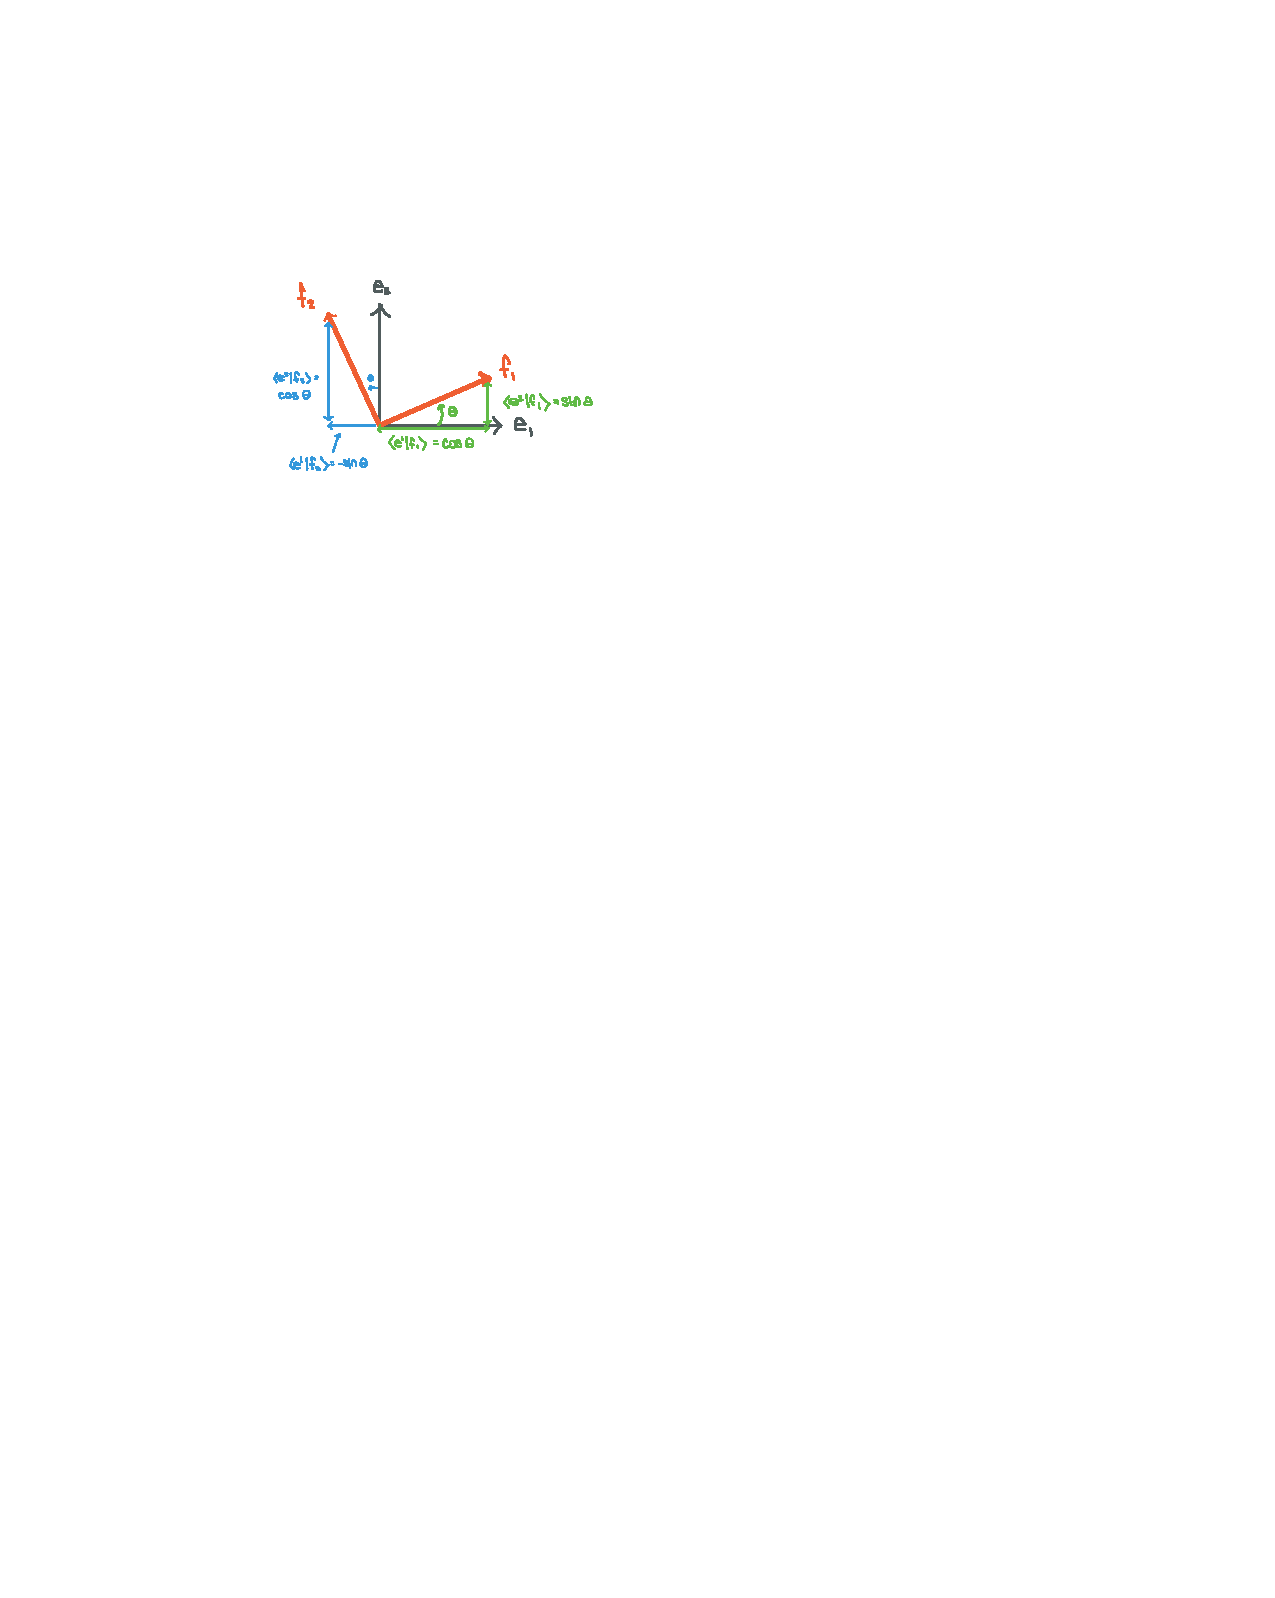
\includegraphics[width=\textwidth]{figures/basis_change_ef.pdf}
    \captionsetup{font={scriptsize,sf}}
    \caption{Components of $(R\inv)\aij{i}{a}$ in \eqref{eq:rotation:from:bra:ket:inv} understood as a projection.}
    \label{fig:basis:change:ef}
\end{marginfigure}
The numbers $\la e^i \mid f_a\ra$ are the \emph{projection} each $f$-basis vector $\ket{f_a}$ onto its $\ket{e_i}$ components. Let us take a moment to pause here: we say it is a projection because $\la e_i, v\ra$ is the component vector $\ket{v}$ in the $\ket{e_i}$ basis direction. But we also argued in \eqref{eq:basis:dual:vectors:as:inner:prod} that $\bra{e^i}$ can be \emph{defined} by $\bra{e^i} \defeq \la e_i , \Vtextvisiblespace[1em]{} \ra$. Thus $\la e^i \mid f_a\ra$ is simply asking what is the component of $\ket{f_a}$ in the $\ket{e_i}$ direction. In Figure~\ref{fig:basis:change:ef} we write out these components. Because all of the vectors are normalized, the projections are all sines and cosines with the appropriate signs.

\begin{marginfigure}%[th]
    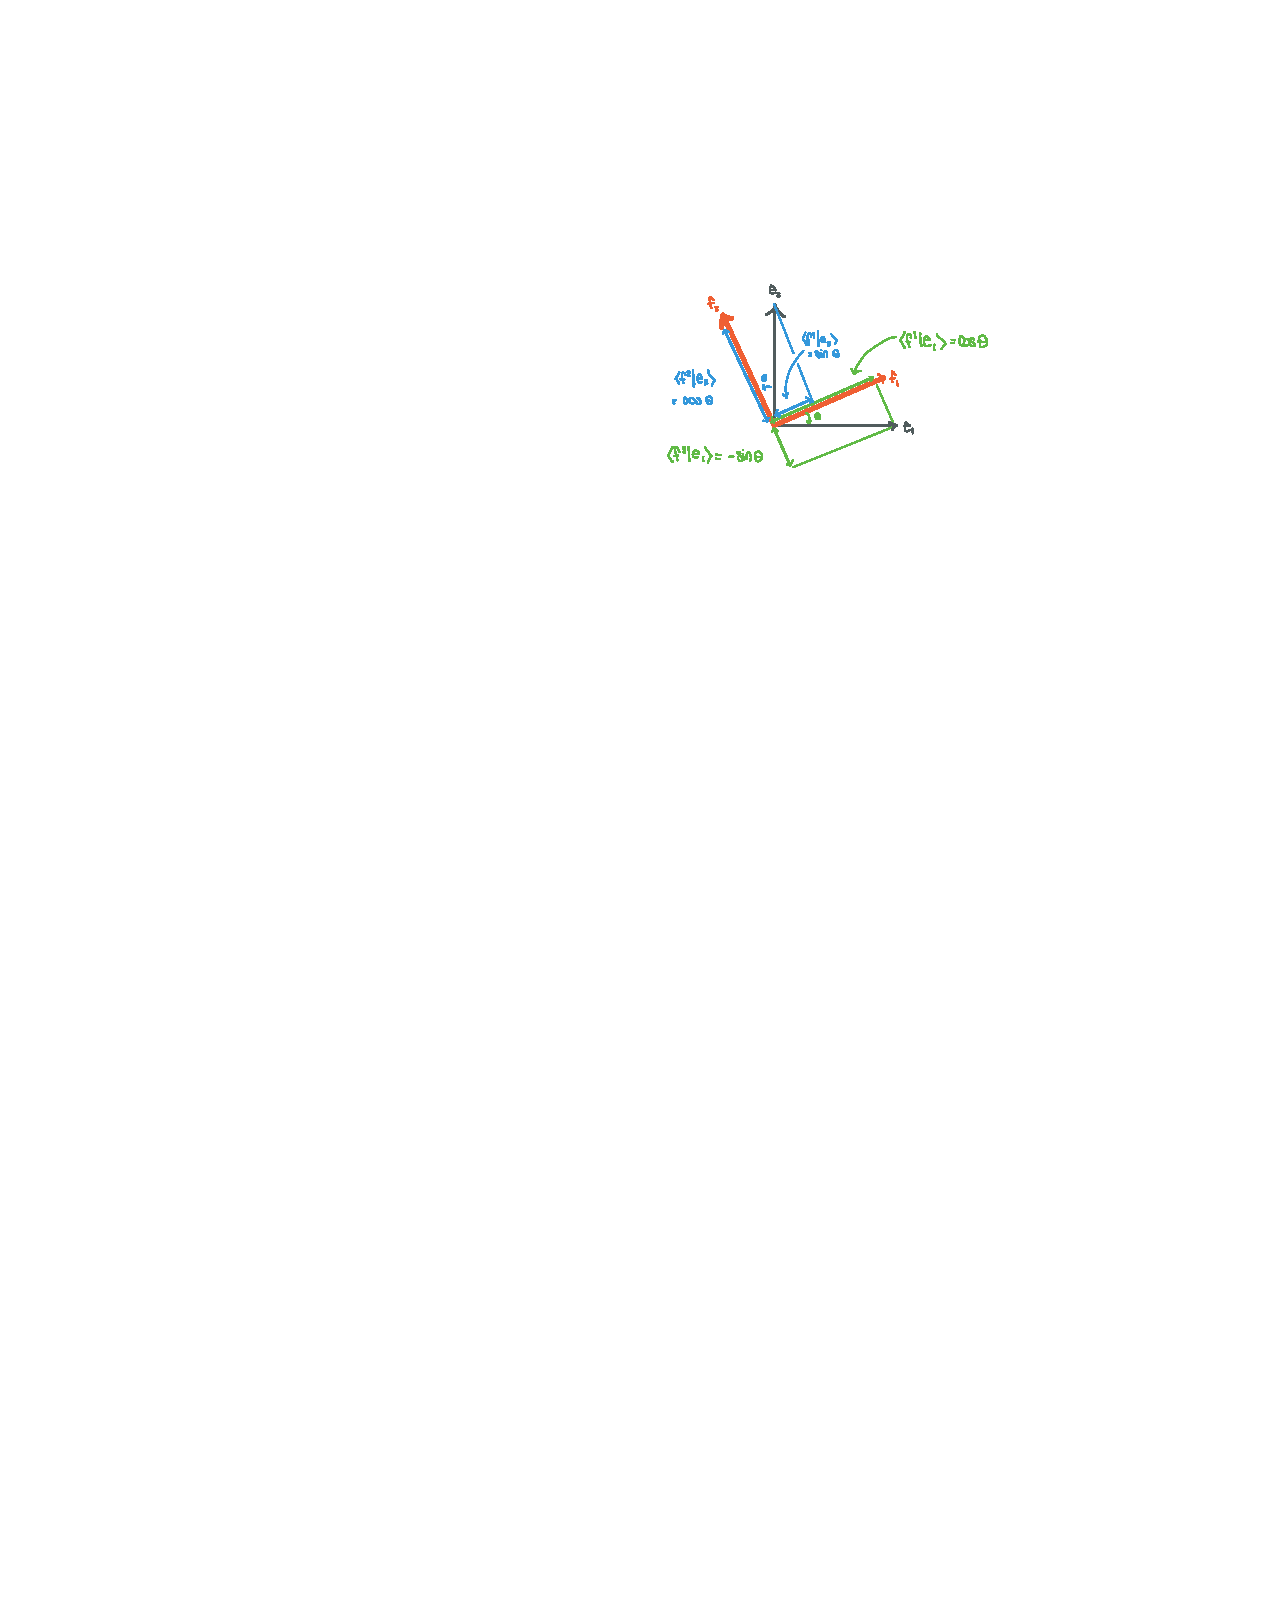
\includegraphics[width=\textwidth]{figures/basis_change_fe.pdf}
    \captionsetup{font={scriptsize,sf}}
    \caption{Components of $R\aij{a}{i}$ in \eqref{eq:rotation:from:bra:ket} understood as a projection.}
    \label{fig:basis:change:fe}
\end{marginfigure}

We can do the same analysis for $(R\inv)\aij{i}{a}$ by looking at the components of $\ket{e_i}$ in the $\ket{f_a}$ basis. We show this in Figure~\ref{fig:basis:change:fe}. Please appreciate that the picture should make it clear that the rotation to go from $\ket{f_a}$ to $\ket{e_i}$ is the `opposite' to that of the rotation to from from $\ket{e_i}$ to $\ket{f_a}$. You can just think about changing the sign of the rotation parameter $\theta$. 

\begin{exercise}
Take a moment to build up the familiarity that $\la f^a \mid e_i$ and $\la e^i \mid f_a$ are components of rotation matrices between bases. Which one rotates from $\ket{f_a}$ to $\ket{e_i}$? Which one goes in the opposite direction? 
\end{exercise}

\begin{exercise}
[\emph{This problem is rather challenging but perhaps enlightening if you can put the time in to do it.}] Redo everything in the last few sections for the case of a Minkowski metric. How are the bras related to the kets? What does the completeness relation look like? How do  you determine  components of the `rotation' matrices (now known as Lorentz transformations)?
\end{exercise}

\begin{subappendices}
\section{Rotations in Three-Dimensions}

In $\RR ^3$ there are three different axes about which we can perform a rotation. These roughly correspond to three rotation matrices:
\begin{align}
    R_1(\theta_1)
    &=
    \begin{pmatrix}
        1 & 0 & \pp 0 \\
        0 & \text{c}_{\theta_1} & -\text{s}_{\theta_1} \\
        0 & \text{s}_{\theta_1} & \pp \text{c}_{\theta_1}
    \end{pmatrix}
    \\
    R_2(\theta_2)
    &=
    \begin{pmatrix}
        \pp \text{c}_{\theta_2} & 0 & \text{s}_{\theta_2} \\
        \pp 0 & 1 & 0 \\
        -\text{s}_{\theta_2} & 0 & \text{c}_{\theta_2}
    \end{pmatrix}
    \\
    R_3(\theta_3)
    &=
    \begin{pmatrix}
        \text{c}_{\theta_3} & -\text{s}_{\theta_3} & 0 \\
        \text{s}_{\theta_3} & \pp\text{c}_{\theta_3} & 0 \\
        0 & \pp 0 & 1
    \end{pmatrix} \ .
    \label{eq:rotation:matrix:basic}
\end{align}
You can see how these break down into two-dimensional rotations along each respective axis. If that is not obvious, please do the following exercise.
\begin{exercise}
Write the transformation of a three-component vector $\vec{v}$ with components $v^i$ under reach of the transformations in \eqref{eq:rotation:matrix:basic}. 
\end{exercise}
Additional rotations are produced by taking products of $R_1$, $R_2$, and $R_3$ by appropriate amounts. The properties of these rotations are outside the scope of our course, but their study is a big part of physics and is known as the \emph{representation theory of Lie groups}. If you want to do a deeper dive into rotation matrices in three dimensions, I recommend Howie Haber's lecture notes for Physics 216 at \acro{UCSC}\footnote{\url{http://scipp.ucsc.edu/~haber/ph216/rotation_12.pdf}}. 


All this is to say that there are more options for rotations in three dimensions. Given a particular rotation, $R$, then the tensor transformation rule in Rule~\ref{idea:transformation:of:upper:and:lower:indices} holds. In fact, one can start to piece together what a rotation in even higher dimensions looks like. You extend the list \eqref{eq:rotation:matrix:basic} to include rotations about every plane---where the plane is simply defined by the two components of the vector that are being mixed into each other. That gives you the list of rotations about each axis. A general rotation is a product of the rotation-about-a-given-axis. Now you know how to manipulate tensors in arbitrary dimensions. Not bad.

\begin{exercise}
One thing to notice is that the order in which you apply rotations matters. Explicitly perform the matrix multiplication on each side of the following non-equation to confirm this:
\begin{align}
    R_1(\theta_1) R_2(\theta_2) \neq R_2(\theta_2) R_1(\theta_1) \ .
\end{align}
We say that the rotation matrices along different axes do not \textbf{commute} because the order in which they are applied matters. This is demonstrated in Fig.~\ref{fig:rotate:QFT}.
\end{exercise}

% non commutivity

\begin{figure}[tb]
    \centering
    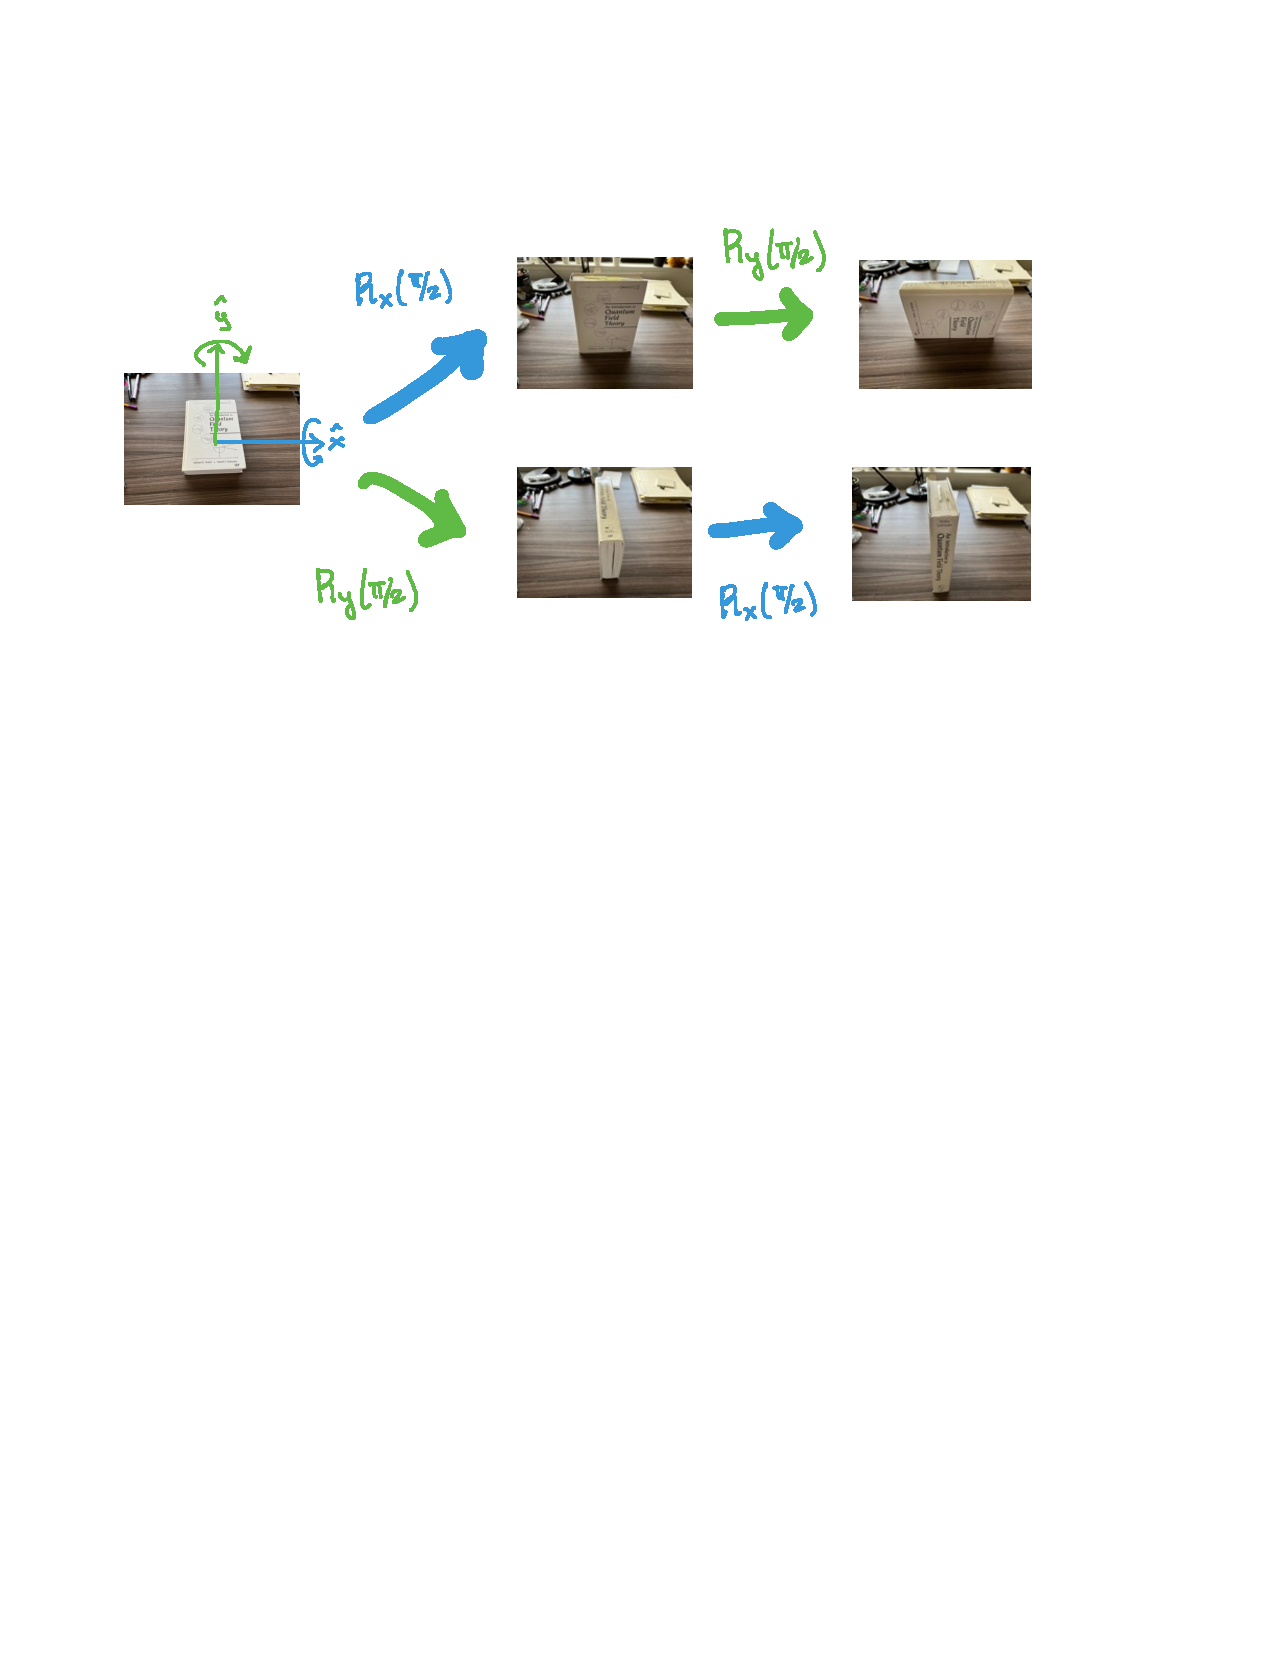
\includegraphics[width=.9 \textwidth]{figures/rotation_qft_sm.pdf}
    \caption{Example of the non-commutativity of rotations. Consider this copy of Peskin and Schr\"oder's \emph{Introduction to Quantum Field Theory}. Orient the $\hat x$ axis in the horizontal direction along the desk and the $\hat y$ axis in the vertical direction along the desk. Performing a $\pi/2$ rotation in the $\hat x$ direction then in the $\hat y$ direction (upper path) gives a different result than performing the rotations in the opposite order (lower path).}
    \label{fig:rotate:QFT}
\end{figure}

\begin{exercise}
Show that the determinant of each of the rotations in \eqref{eq:rotation:matrix:basic} is one. Argue that a general rotation in three dimensions, which is a product of these rotations, also has determinant equal to one. Argue further that the determinant of a rotation in any number of dimensions is equal to one.
\end{exercise}

\section{Invariance of Trace and Determinant}

The trace and the determinant of a matrix are invariant under rotations. This may sound trivial\footnote{``Trivial'' is the mathematical translation of when I say `obvious.'}: they are numbers with no indices, and numbers with no indices do not transform under rotations. The relevance of the invariance of the trace and determinant are that they are numbers that are formed out of the components of a matrix that do not transform, even though the components of a matrix, $M\aij{i}{j}$, \emph{do} transform under a rotation. 

\subsection{Trace}

Let us see that this is the case. Under a rotation, the trace of a matrix, $M\aij{i}{j}$ transforms as:
\begin{align}
    M\aij{i}{j} \to (M')\aij{i}{i} = R\aij{i}{k} M\aij{k}{\ell} (R\inv)\aij{\ell}{i} \ .
\end{align}
We have started writing $R$ instead of $R(\theta)$ since we generalize to the case of higher-dimensional rotations with more than one parameters. Now we're going to do something sneaky. Let us move the $(R\inv)\aij{\ell}{i}$ factor around on the right-hand side. We made a big deal in \eqref{eq:multiplication:MN:indices} that we are allowed to do this \emph{as long as we keep the indices the same}:
\begin{align}
    (M')\aij{i}{i}
    =
    (R\inv)\aij{\ell}{i} R\aij{i}{k} M\aij{k}{\ell} 
    = (R\inv\, R)\aij{\ell}{k} M\aij{k}{\ell} 
    = \delta^\ell_k M\aij{k}{\ell} 
    = M\aij{k}{k} \ . 
\end{align}
Did you see what we did? We noticed that because the last index of $(R\inv)\aij{\ell}{i}$ matches the first index of $R\aij{i}{k}$, these two matrices are actually being multiplied in the expression for the trace. In other words, we have derived the following matrix-level expression:
\begin{align}
    \Tr R M R\inv = \Tr R\inv R M = \Tr M \ .
\end{align}
\begin{exercise}
Check that the above argument holds for the trace of any product of matrices, not necessarily rotations:
\begin{align}
    \Tr ABC = \Tr CAB = \Tr BCA \ .
\end{align}
We call this a \emph{cyclic permutation} of the product $ABC$.
\end{exercise}
I hope you are starting to appreciate the utility of the index notation.

\subsection{Determinant}

Moving on to the determinant, we appeal a couple of rules that we motivate in Chapter~\ref{ch:determinant}, see Section~\ref{sec:determinant:of:product},
\begin{align}
    \det(MN) &= (\det M)(\det N)
    &
    \det(M\inv ) &= (\det M)\inv  \ .
\end{align}
Then it is straightforward to read off that
\begin{align}
    \det M \to \det M' = \det(RMR\inv ) = \det M\ \frac{\det R}{\det R} = \det M \ .
\end{align}
In Chapter~\ref{ch:determinant} we define the determinant as a volume of a parallelpiped. Rotations do not change the volume of a parallelpiped . Rotating a mug does not change the capacity of the mug, though it may cause its contents to spill out. 

\end{subappendices}
